\chapter{Installer le logiciel}

\section{Consultez la documentation du framework !}

Le logiciel a été conçu à partir du framework \textit{Prototypephp}. La documentation associée \cite{pphp-doc} récapitule l'ensemble des informations nécessaires pour réaliser l'installation générale (configuration du serveur, définition des droits d'accès, etc.).

De nombreuses passages ont été repris ici, mais il n'est pas inutile de se référer au document d'origine. 

\section{Configurer le serveur}

L'application est conçue pour fonctionner à partir d'une adresse unique de type : {\NoAutoSpacing\textit{https://monsite.com}}. Le chiffrement est obligatoire (protocole https). Il n'est pas possible d'installer l'application dans un sous-dossier, par exemple : {\NoAutoSpacing \textit{https://monsite.com/collec-science}} ne fonctionnera pas.

Un script d'installation quasi-automatique est disponible et permet :
\begin{itemize}
\item d'installer les paquetages nécessaires (Apache, PHP, Postgresql principalement) ;
\item de télécharger la dernière version de l'application ;
\item de créer la base de données, avec mise en place d'une sauvegarde automatique ;
\item de pré-configurer le serveur pour qu'il soit prêt à être utilisé.
\end{itemize}

Pour déployer une nouvelle instance, une fois le serveur installé, dans un terminal, tapez les commandes suivantes :
\begin{lstlisting}
wget https://github.com/Irstea/filo-science/install/deploy_new_instance.sh
sudo -s
./deploy_new_instance.sh
\end{lstlisting}

Suivez les messages affichés à l'écran. Vous devrez notamment modifier le fichier :
\begin{lstlisting}
/etc/apache2/sites-available/filo-science.conf 
\end{lstlisting}
pour indiquer l'adresse DNS utilisée pour accéder à l'application et le certificat de chiffrement associé.

La configuration a été réalisée pour un serveur Linux fonctionnant avec Ubuntu 16.04 LTS Server ou Debian 9. Elle peut bien sûr être adaptée à d'autres distributions Linux. Par contre, rien n'a été prévu pour faire fonctionner l'application directement dans une plate-forme windows, même si, en théorie, cela devrait être possible.

\subsection{Configurer Apache}
Les modules suivants doivent être activés :
\begin{lstlisting}
a2enmod ssl
a2enmod headers
a2enmod rewrite
\end{lstlisting}
\subsection{Modules PHP nécessaires}
Modules complémentaires nécessaires :
\begin{itemize}
\item \textit{php-mbstring}
\item \textit{php-pgsql}
\item \textit{php7.0-xml} 
\item \textit{php-xdebug} pour les phases de mise au point
\item \textit{php-curl} pour l'identification via un serveur CAS.
\end{itemize}

Le stockage et l'affichage des photos nécessite :
\begin{itemize}
\item \textit{php-imagick}
\end{itemize}


\subsection{Configurer l'hôte virtuel et SSL}
L'application ne fonctionne qu'en mode SSL, les cookies de session n'étant pas transmis sur des liens non chiffrés. Vous devrez modifier le paramétrage proposé dans le fichier install/apache2/filo-science.conf, pour indiquer notamment le nom du certificat utilisé et le nom du site.

\subsubsection{Cas particulier de l'identification en mode HEADER}

Si vous identifiez vos utilisateurs derrière un proxy d'identification, comme Lemon\-Ldap par exemple, vous devrez limiter l'accès de l'application uniquement au proxy. La commande \textit{Directory} devient donc :
\begin{lstlisting}
    <Directory /var/www/html>
        Options FollowSymLinks MultiViews
        AllowOverride all
        Order allow,deny
        allow from 10.1.2.3
    </Directory>

\end{lstlisting}
\textit{10.1.2.3} correspond à l'adresse IP du serveur proxy d'identification.

\subsection{Configurer le dossier d'installation}

Le principe général est que le dossier contenant l'application contient, dans son nom, le numéro de version (v2.0 par exemple), et un lien virtuel (filo-science) pointe vers celui-ci. C'est le lien qui est la cible de l'adresse web : ainsi, à chaque nouvelle version, il suffit de mettre à jour le code de l'application et de faire pointer le lien vers le nouveau dossier pour que celle-ci soit opérationnelle.

Des scripts seront fournis pour réaliser automatiquement les mises à jour (dans le cas d'installations mono-instances).

\subsubsection{Cas général : une seule instance hébergée dans le serveur}

Utilisez le script fourni, qui créera automatiquement les dossiers nécessaires. 


\subsubsection{Cas particulier : faire cohabiter plusieurs instances avec le même code}
\label{dnsmultiple}
Il est possible d'utiliser le même code applicatif pour alimenter des bases de données différentes (ou des données stockées dans des schémas différents). Cette fonctionnalité est basée sur l'attribution d'entrées DNS différentes. 

Le mécanisme est décrit dans la figure \ref{dnsmultipleschema} \textit{\nameref{dnsmultipleschema}}, page \pageref{dnsmultipleschema}.

\begin{figure}[H]
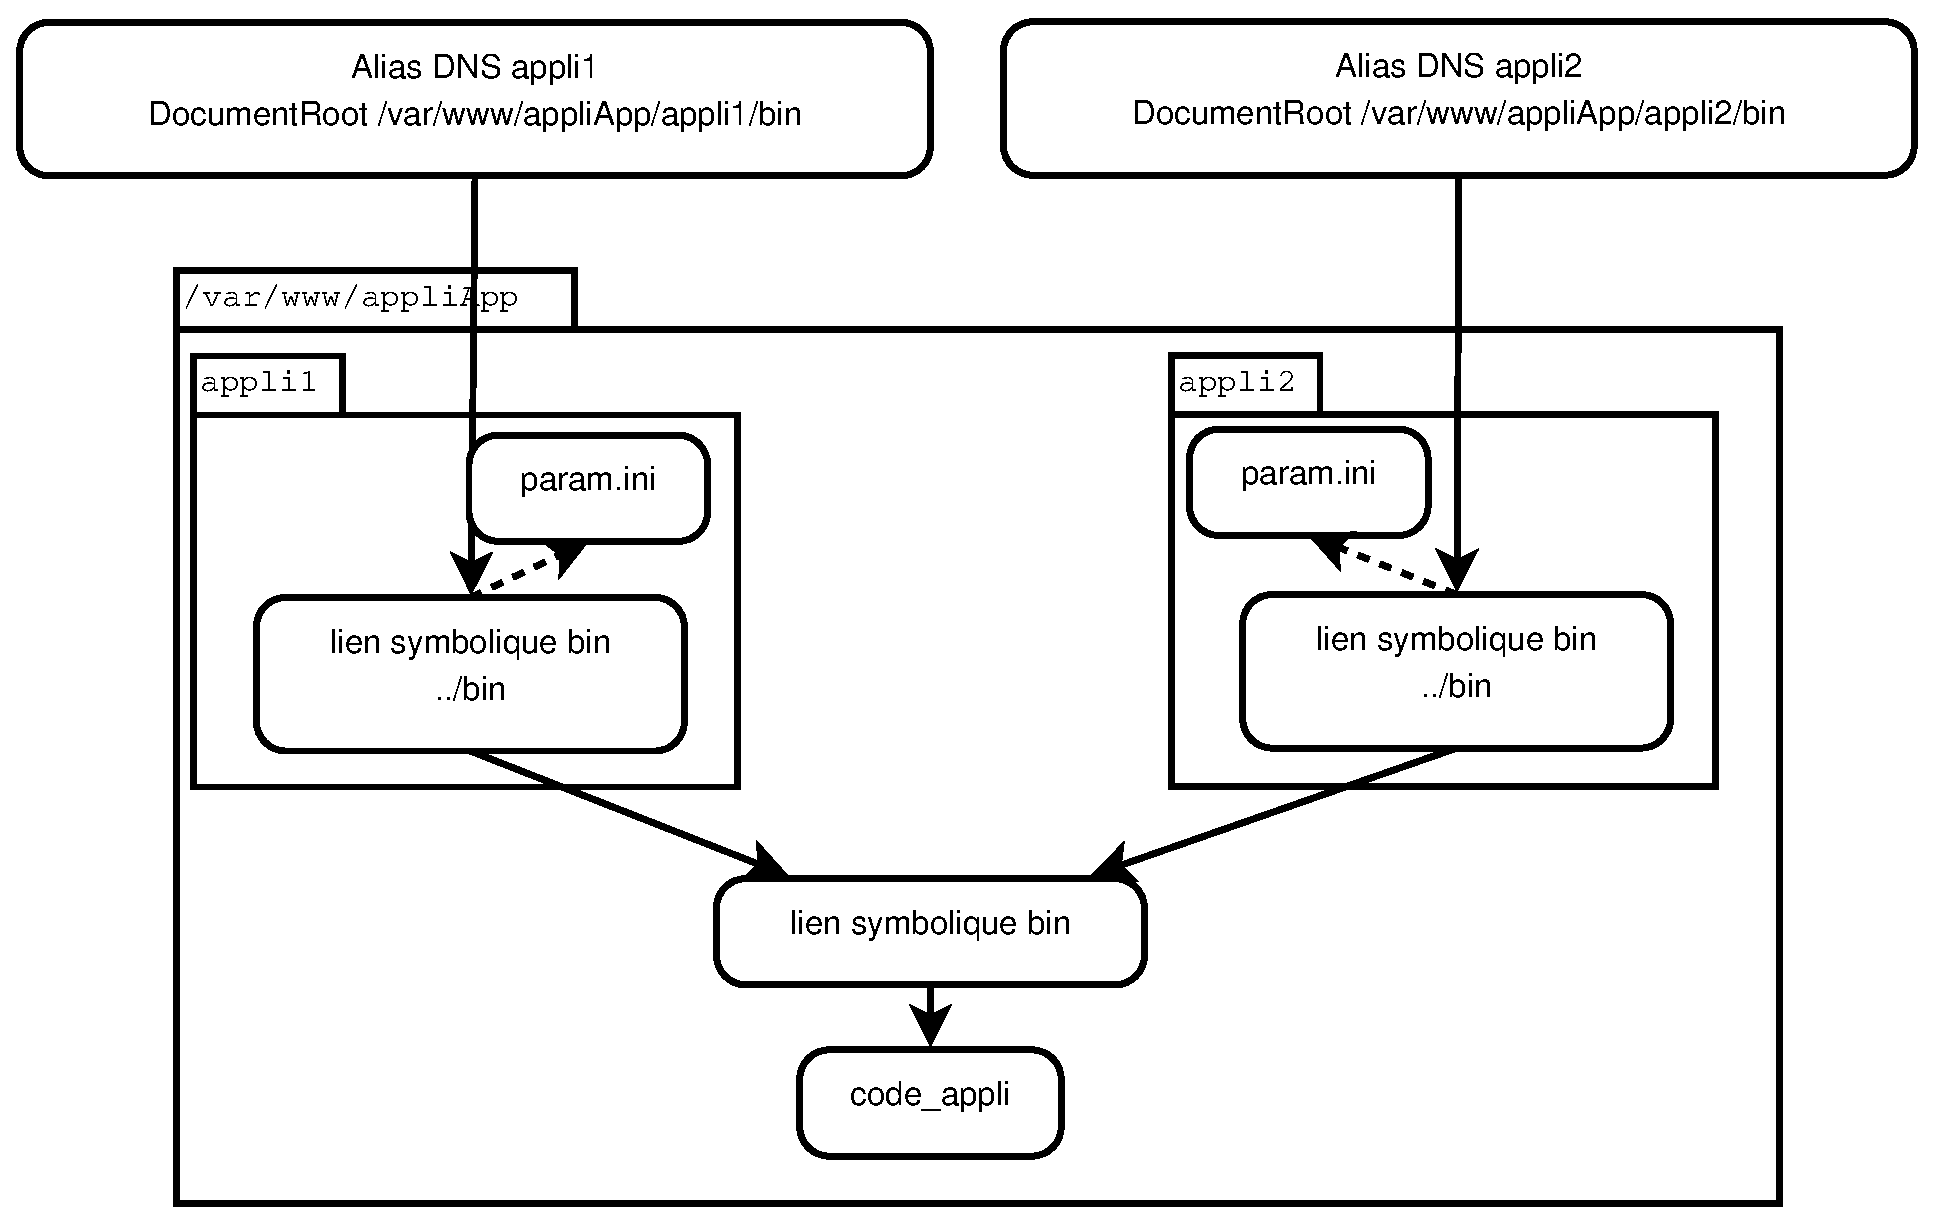
\includegraphics[width=\linewidth]{images/dnsmultiple}
\caption{\label{dnsmultipleschema}Schéma général d’implémentation pour utiliser le même code avec des noms d’application et des jeux de données différents}
\end{figure}

Dans le paramétrage de l’alias DNS (en principe, dans \textit{/etc/apache2/sites-available}), l’application pointe vers le dossier \textit{/var/www/appliApp/appli1/bin}. \textit{/var/www} correspond à la racine du site web, \textit{appliApp} au dossier racine de l’application, \textit{appli1} au dossier spécifique de l’alias DNS. Ce dossier \textit{appli1} ne contient que deux fichiers : \textit{param.ini}, qui contient les paramètres spécifiques, et \textit{bin}, qui est un lien symbolique vers le dossier \textit{../bin}.

Le dossier \textit{../bin} (donc, dans\textit{ /var/www/appliApp}) est lui aussi un alias qui pointe vers le code réel de l’application, ici \textit{code\_appli}. Le fichier \textit{param.inc.php} doit contenir les commandes suivantes pour que le fichier \textit{param.ini} soit correctement chargé selon le contexte :
\begin{lstlisting}
$chemin = substr($_SERVER["DOCUMENT_ROOT"],0, strpos($_SERVER["DOCUMENT_ROOT"],"/bin"));
$paramIniFile = "$chemin/param.ini";
\end{lstlisting}

Le fichier \textit{param.ini} sera cherché dans le dossier parent du code de l’application, c’est à dire soit dans \textit{appli1}, soit dans \textit{appli2} dans cet exemple. Il suffit qu’il contienne les paramètres adéquats pour rendre l’application utilisable dans des contextes différents à partir du même code initial.

Le fichier \textit{param.ini} est le dernier qui est traité par l'application pour récupérer les paramètres. Ceux-ci sont lus dans l'ordre suivant :

\textbf{param/param.default.inc.php $\rightarrow$ param/param.inc.php $\rightarrow$ ../param.ini}

\textit{param.ini} contiendra les entrées spécifiques liées au DNS utilisé pour accéder à l'application, en principe tout ou partie de celles-ci :
\begin{lstlisting}
BDD_schema=filo-science, public, gacl
BDD_login=compte_de_connexion
BDD_passwd=mot_de_passe_de_connexion
BDD_dsn=pgsql:host=serveur;dbname=base_de_donnees;sslmode=require
GACL_aco=filo
\end{lstlisting}

Si un libellé contient une apostrophe, la chaîne doit être insérée dans des guillemets doubles, comme ici pour la variable \textit{APPLI\_titre}.


\subsection{Droits à attribuer au serveur web}
\label{droitsApache}
Le serveur web doit pouvoir accéder en lecture à l'ensemble des fichiers de l'application, et en écriture à deux dossiers :
\begin{itemize}
\item \textit{display/templates\_c} : fichier utilisé par Smarty pour compiler les modèles de documents HTML ;
\item \textit{img} : dossier de génération des images et des fichiers temporaires.
\end{itemize}

Deux scripts sont fournis pour attribuer les droits : 
\begin{itemize}
\item \textbf{install/apache2/upgrade\_rights.sh} : positionne les droits en utilisant les droits standards Linux (owner, group)
\item \textbf{install/apache2/upgrade\_rights\_with\_acl.sh} : positionne les droits à partir des ACL.
\end{itemize}

Les scripts doivent être lancés ainsi :
\begin{lstlisting}
filo-2.0/install/apache2/upgrade_rights.sh v2.0
\end{lstlisting}
ou 
\begin{lstlisting}
filo-2.0/install/apache2/upgrade_rights_with_acl.sh v2.0
\end{lstlisting}


\section{Configurer l'application}

L'application est configurable par l'intermédiaire de trois fichiers :

\textbf{param/param.default.inc.php $\rightarrow$ param/param.inc.php $\rightarrow$ ../param.ini}

Le premier fichier contient les paramètres par défaut. Il est systématiquement fourni à chaque nouvelle version de l'application.

Le second est spécifique de l'implémentation. Il comprend notamment les informations liées à la connexion à la base de données, à la méthode d'identification, ou à la recherche des attributs dans l'annuaire LDAP. 

le troisième est destiné à offrir la possibilité d'accéder, à partir du même code applicatif, à plusieurs bases de données différentes (\textit{cf.} \ref{dnsmultiple} \textit{\nameref{dnsmultiple}}, page \pageref{dnsmultiple}).

Voici les principaux paramètres utilisés :

\subsection{Connexion à la base de données}

Dans la pratique, deux connexions sont nécessaires : l'une pour accéder à la base des droits, l'autre aux données proprement dites. Voici les paramètres à définir :

\begin{longtable}{|p{4cm}|p{11cm}|}
\hline
\textbf{Variable} & \textbf{Signification} \\
\hline
\endhead
BDD\_login & compte de connexion à la base de données \\
\hline
BDD\_passwd & mot de passe associé\\
\hline
BDD\_dsn & adresse de la base de données sous forme normalisée\\
\hline
BDD\_schema & schéma utilisé (plusieurs schémas peuvent être décrits, en les séparant par une virgule - fonctionnement propre à Postgresql)\\
\hline
GACL\_dblogin & compte de connexion à la base de données des droits\\
\hline
GACL\_dbpasswd & mot de passe associé\\
\hline
GACL\_dsn & adresse normalisée \\
\hline
GACL\_schema & schéma utilisé\\
\hline
GACL\_aco & nom du code de l'application utilisé dans la gestion des droits\\
\hline
\caption{Variables utilisées pour paramétrer les connexions}
\end{longtable}

\subsection{Identification des utilisateurs}

\begin{longtable}{|p{6cm}|p{10cm}|}
\hline
\textbf{Variable} & \textbf{Signification} \\
\hline
\endhead
ident\_type & Type d'identification supporté. L'application peut gérer \textbf{BDD} (uniquement en base de données),\textbf{LDAP} (uniquement à partir d'un annuaire LDAP) \textbf{LDAP-BDD} (d'abord identification en annuaire LDAP, puis en base de données), \textbf{CAS} (serveur d'identification \textit{Common Access Service}\footnote{serveur externe gérant l'identification des utilisateurs, et renvoyant à l'application le login utilisé}), et enfin \textbf{HEADER} (identification derrière un proxy qui fournit le login dans une variable d'entête HTTP)\\
\hline
CAS\_plugin & Nom du plugin utilisé pour une connexion CAS \\
\hline
CAS\_address & Adresse du serveur CAS\\
\hline
CAS\_port & Systématiquement 443 (connexion chiffrée)\\
\hline
CAS\_CApath & chemin d'accès au certificat du serveur CAS \\
\hline
LDAP & tableau contenant tous les paramètres nécessaires pour une identification LDAP \\
\hline
ident\_header\_login\_var & par défaut, AUTH\_USER. Nom de la variable qui contiendra le login dans le cas d'une identification en mode HEADER (le radical HTTP\_  ne doit pas être indiqué) \\
\hline
privateKey & clé privée utilisée pour générer les jetons d'identification (ré-identification automatique après une première connexion) \\
\hline
pubKey & clé publique utilisée pour générer les jetons d'identification \\
\hline
tokenIdentityValidity & durée de validité, en secondes, des jetons d'identification\\
\hline
MAIL\_enabled & Si à 1, l'envoi de mail est géré par l'application \\
\hline
CONNEXION\_max\_attemps & nombre maximum d'essais de connexion avant blocage temporaire du compte \\
\hline
CONNEXION\_blocking\_duration & durée de blocage du compte \\
\hline
APPLI\_mailToAdminPeriod & intervalle de temps entre l'envoi d'un mail de notification de blocage de compte à un administrateur \\
\hline
APPLI\_admin\_ttl & durée de vie d'une session d'administration (temps maximum entre deux accès à une page d'administration avant réidentification) \\
\hline
APPLI\_lostPassword & Si à 1, autorise la récupération du mot de passe perdu, par envoi d'un mail avec un lien chiffré. Nécessite également que MAIL\_enabled soit positionné à 1 \\
\hline

\caption{Variables utilisées pour paramétrer l'identification}
\end{longtable}

\subsubsection{Ré-identification par jeton}

L'application permet de conserver l'identification plus longtemps que celle définie dans le serveur, en rejouant la connexion avec un jeton d'identification chiffré. Cela évite, par exemple, de devoir se ré-identifier toutes les heures si on accède au logiciel à partir d'un terminal mobile (smartphone ou tablette, par exemple).

Les trois dernières variables permettent de configurer ce mode d'identification. 

Le framework peut générer un jeton chiffré après la première identification, qui sera analysé pour savoir si l'utilisateur peut être ré-identifié automatiquement.

Pour que ce mécanisme fonctionne, il faut :
\begin{itemize}
\item que le paramètre \textit{tokenIdentityValidity} ait une durée de validité supérieure à la durée de vie de la session. Il est raisonnable de ne pas fixer une durée de vie supérieure à une journée de travail (10 heures). Le cookie transmis est protégé ;
\item que les clés privée et publique, utilisées pour le chiffrement du jeton, soient accessibles au serveur web (variables \textit{privateKey} et \textit{publicKey}).
\end{itemize}

Les clés sont générées automatiquement avec le script d'installation automatique du serveur et de l'application.

Le jeton est chiffré avec la clé privée, ce qui lui permet d'être lu, le cas échéant, par l'application. Il contient le login et la date d'expiration. 

Si l'utilisateur déclenche une déconnexion, le jeton est supprimé.

Pour plus d'informations, consultez comment fonctionne le mécanisme de ré-identification par jeton \cite{token}.

\subsubsection{Identification par HEADER}

Dans ce mode d'identification, le serveur web est placé derrière un serveur d'identification, appelé proxy d'identification. L'adresse de l'application pointe vers ce dernier. 

Le proxy gère la connexion de l'utilisateur, et fournit à l'application le login dans une variable configurable. Cette variable est accessible dans le tableau \$\_SERVER, par exemple \$\_SERVER [ "HTTP\_AUTH\_USER" ].

Pour activer ce mécanisme, il faut modifier les paramètres suivants dans le fichier \textit{param.ini.php} :
\begin{lstlisting}
$ident_type = "HEADER";
$ident_header_login_var = "AUTH_USER";
\end{lstlisting}

la variable ne doit pas contenir la racine HTTP\_ (une fonction l'extrait automatiquement).

\subsection{Configuration de l'accès à l'annuaire LDAP}

Les paramètres LDAP sont stockés dans un tableau :
\begin{lstlisting}
$LDAP = array(
		"address"=>"localhost",
		"port" => 389,
		"rdn" => "cn=manager,dc=example,dc=com",
		"basedn" => "ou=people,ou=example,o=societe,c=fr",
		"user_attrib" => "uid",
		"v3" => true,
		"tls" => false,
		"groupSupport"=>true,
		"groupAttrib"=>"supannentiteaffectation",
		"commonNameAttrib"=>"displayname",
		"mailAttrib"=>"mail",
		'attributgroupname' => "cn",
		'attributloginname' => "memberuid",
		'basedngroup' => 'ou=example,o=societe,c=fr'
);
\end{lstlisting}


L'application peut non seulement identifier les utilisateurs auprès de l'annuaire LDAP, mais également récupérer les groupes auxquels ils appartiennent dans celui-ci.

Voici les paramètres à indiquer dans ce cas de figure (valable en principe pour tout annuaire compatible OpenLdap) : 
\begin{longtable}{|p{4cm}|p{11cm}|}
\hline
\textbf{Variable} & \textbf{Signification} \\
\hline
\endhead
address &  adresse de l'annuaire\\
\hline
port & 389 en mode non chiffré, 636 en mode chiffré\\
\hline
rdn & compte de connexion, si nécessaire \\
\hline
basedn & base de recherche des utilisateurs\\
\hline
user\_attrib & nom du champ contenant le login à tester\\
\hline
v3 & toujours à \textit{true}\\
\hline
tls & \textit{true} en mode chiffré\\
\hline
groupSupport & \textbf{true} si l'application recherche les groupes d'appartenance du login dans l'annuaire\\
\hline
groupAttrib & Nom de l'attribut contenant la liste des groupes d'appartenance\\
\hline
commonNameAttrib & Nom de l'attribut contenant le nom de l'utilisateur\\
\hline
mailAttrib & Nom de l'attribut contenant l'adresse mail de l'utilisateur\\
\hline
attributgroupname & Attribut contenant le nom du groupe lors de la recherche des groupes (cn par défaut)\\
\hline
attributloginname & attribut contenant les membres d'un groupe\\
\hline
basedngroup & base de recherche des groupes \\
\hline
\caption{Variables utilisées pour paramétrer l'accès à l'annuaire LDAP}
\end{longtable}

\subsection{Paramètres spécifiques}
\label{paramspec}

\begin{longtable}{|p{4cm}|p{11cm}|}
\hline
\textbf{Variable} & \textbf{Signification} \\
\hline
\endhead
APPLI\_photoStockage & dossier contenant les photos générées par l'application, avant transmission au navigateur. Par défaut : \textit{img}\\
\hline
APPLI\_maxfilesize & Taille maximale des photos téléchargeables. Par défaut : 100000000 \\
\hline

\caption{Variables spécifiques}
\end{longtable}

\subsection{Paramètres stockés en base de données}
\label{paramdb}

À partir de la version 2, certains paramètres peuvent être stockés dans la base de données, pour éviter qu'ils ne soient dépendants de la configuration du serveur.

Ces paramètres sont accessibles depuis le menu \textit{administration}, item \textit{Paramètres de l'application}.

Voici la liste des paramètres actuellement décrits :
\begin{longtable}{|p{4cm}|p{11cm}|}
\hline
\textbf{Variable} & \textbf{Signification} \\
\hline
\endhead
APPLI\_title & Titre de l'application tel qu'il figure entre l'icône et le menu\\
\hline
mapDefaultLat & Latitude de positionnement par défaut des cartes \\
\hline
mapDefaultLong & Longitude de positionnement par défaut des cartes \\
\hline
mapDefaultZoom & Niveau de zoom des cartes par défaut \\
\hline
\caption{Paramètres stockés dans la base de données}
\end{longtable}


\section{Créer la base de données}

La base de données est composée de deux schémas : l'un pour stocker les informations d'identification, les droits d'accès et les traces (gacl), l'autre pour les données proprement dites (filo).

Le schéma \textit{public} ne devrait jamais être utilisé pour stocker l'information : réservez-le pour les composants communs, comme Postgis.

Les tables de gestion des droits peuvent être communes à plusieurs jeux / applications différentes : la variable \textit{GACL\_aco} permet de séparer la gestion des droits pour chaque application, tout en travaillant à partir des mêmes utilisateurs (répartis le cas échéant dans des groupes différents selon le jeu de données considéré).

Les tables sont créées à partir du script \textit{install/pgsql/create\_db.sql}.


Un compte d'administration par défaut est créé automatiquement :
\begin{itemize}
\item login : \textbf{admin}
\item mot de passe : \textbf{password}
\end{itemize}

Il devra être supprimé quand un autre compte d'administration aura été créé.


\subsection{Login de connexion}

Si la base de données et l'application sont hébergés dans deux serveurs différents, il est fortement conseillé de créer deux logins de connexion, un pour le schéma des droits, l'autre pour les schémas applicatifs. Ces logins ne doivent pouvoir être utilisés que depuis le serveur web hébergeant l'application.

Cette opération est possible en modifiant le fichier \textit{/etc/postgresql/9.5/main/pg\_hba.conf} selon ce principe :

\begin{lstlisting}
# Connexions pour les serveurs web 
host nom_database userGacl adresse_serveur/32 md5 
host nom_database userData adresse_serveur/32 md5
\end{lstlisting}

Le login utilisé dans \textit{userGacl} correspond à la variable \textit{\$GACL\_dblogin}, et \textit{userData} à \textit{\$BDD\_login}.

et en rechargeant ensuite la configuration de Postgresql avec la commande :
\begin{lstlisting}
service postgresql reload
\end{lstlisting}

\subsection{Droits sur les tables}

Le compte utilisé pour la connexion au schéma des droits doit pouvoir modifier les informations présentes dans l'ensemble des tables de \textit{gacl}. Il ne devrait pas pouvoir accéder aux autres schémas (hormis \textit{public}), sauf en cas d'installation mono-serveur (base de données hébergée dans la même machine et connexion à distance impossible).

Le compte utilisé pour accéder aux schémas des données doit pouvoir modifier l'ensemble des informations dans les schémas de données, et lire la table \textit{gacl.aclgroup}.

Le plus simple est d'utiliser le logiciel \textit{pgAdmin} \cite{pgadmin} pour attribuer les droits.

Le script d'installation automatique rend le compte \textit{filo} propriétaire de la base de données, ce qui simplifie la gestion des droits sur les tables.

\subsection{Scripts de modification}

Lors de la livraison de nouvelles versions, il est possible que des scripts de modification soient livrés pour mettre à niveau la base de données. Ces scripts doivent être exécutés dans tous les schémas contenant des données applicatives (pour plus de détails, consultez ci-après \textit{\nameref{newVersion}}).

\section{Mise en production}

Une fois l'application configurée, et après avoir créé un nouveau compte d'administration :
\begin{itemize}
\item supprimez le compte \textit{admin}, livré par défaut, qui ne doit pas être conservé. Sa désactivation n'est pas suffisante : si pour une raison ou pour une autre le compte est réactivé, n'importe qui pourra récupérer les droits totaux ;
\item supprimez le dossier \textit{install} qui contient les scripts de création des tables ;
\item déplacez le dossier \textit{database}, qui contient la documentation d'installation et de configuration (elle n'a pas à rester accessible depuis le site web) ;
\item faites une revue des droits, pour vous assurer que tout est correctement configuré.
\end{itemize}

Vous pouvez également tester si la configuration du serveur est correcte en recourant à \textit{ZAProxy} \cite{zaproxy}, qui analysera la communication entre le serveur et un navigateur et identifiera les problèmes éventuels de non conformité (mauvaise réécriture des entêtes HTML suite à une mauvaise configuration du serveur Apache, par exemple).

\section{Installer une nouvelle version}
\label{newVersion}

\subsection{Faites une sauvegarde de la base de données}
Il arrive fréquemment que la structure de la base de données évolue. Avant toute opération, assurez-vous de disposer d'une sauvegarde, dans un autre support.

Un programme de sauvegarde est disponible dans \textit{install/pgsql/backup.sh}. Vous pouvez l'exécuter manuellement ainsi :
\begin{lstlisting}
su postgres -c "install/pgsql/backup.sh"
\end{lstlisting}

La sauvegarde sera stockée dans \textbf{/var/lib/postgresql/backup}.

Si vous avez utilisé le script d'installation automatique, le programme est également présent dans \textit{/var/lib/postgresql}.

\subsection{Procédure automatique de mise à jour}

Si l'application est installée dans un serveur dédié à cet usage (installation réalisée avec le script \href{https://github.com/Irstea/filo-science/blob/master/install/deploy_new_instance.sh}{https://github.com/Irstea/filo-science/blob/master/install/deploy\_new\_instance.sh}), un script de mise à jour automatique peut être téléchargé. Il est disponible dans le dossier\\ \href{https://github.com/Irstea/filo-science/tree/master/install}{https://github.com/Irstea/filo-science/tree/master/install}, et est sous la forme :
\begin{lstlisting}
upgrade-2.0-2.1.sh
\end{lstlisting}
où \textbf{2.0} correspond à la version courante de votre installation, et \textbf{2.1} à la version cible.

Pour utiliser ce script :
\begin{lstlisting}
sudo -s
wget https://github.com/Irstea/filo-science/raw/master/install/upgrade-2.0-2.1.sh
chmod +x upgrade-2.0-2.1.sh
./upgrade-2.0-2.1.sh
\end{lstlisting}

Le script va télécharger le code de la nouvelle version et mettra à jour la base de données, si c'est nécessaire.

\subsection{Sauvegarder le fichier contenant les paramètres de l'application}

Le fichier \textit{param/param.inc.php} contient vos paramétrages spécifiques. Lors de l'installation d'une nouvelle version, il va être supprimé.

Faites-en une copie, et remettez-le en place après avoir installé la nouvelle version.

\subsection{Consultez le fichier news.txt}

Le fichier \textit{param/news.txt} contient la description des modifications apportées au logiciel. Il précise notamment si une mise à jour de la base de données doit être appliquée.

\subsection{Mise à jour de la structure de la base de données}

Le dossier \textit{install/pgsql} contient les scripts de création et de mise à jour de la base de données. Les scripts de mise à jour sont nommés ainsi :
\begin{lstlisting}
alter_versionAnterieure-versionMiseAJour.sql
\end{lstlisting}

\textit{versionAnterieure} correspond à la version la plus ancienne qui doit être mise à jour, \textit{versionMiseAJour} la version cible. Par exemple :
\begin{lstlisting}
alter_2.0-2.1.sql
\end{lstlisting}
indique que toutes les versions entre \textit{2.0} et \textit{2.1} doivent être mises à jour avec le script indiqué. Si vous avez \og sauté \fg{} certaines versions du logiciel, il est possible que plusieurs scripts doivent être appliqués.

La mise à jour doit être appliquée dans tous les schémas contenant des données, notamment dans le cas où le même logiciel est utilisé pour gérer plusieurs jeux de données.

Avant d'exécuter les scripts, vérifiez leur contenu, et notamment le nom des schémas.

Ne relancez jamais l'exécution d'un script.

\subsection{Reconfigurer les droits d'accès au serveur web}

Après installation de la nouvelle version du code, n'oubliez-pas de reconfigurer les accès en lecture pour le compte utilisé pour faire fonctionner le serveur web, et en écriture pour les dossiers \textit{img} et \textit{display/templates\_c} (\textit{cf.} \ref{droitsApache} \textit{\nameref{droitsApache}}, page \pageref{droitsApache}).

\subsection{Supprimer les dossiers inutiles}
Une fois la mise en production validée, supprimez le dossier \textit{install} et déplacez le dossier \textit{database}, et faites une revue des droits pour vous assurer qu'il n'y a pas eu de modification intempestive ou que la configuration est toujours correcte.

\subsection{Vérifier la configuration du chiffrement}
Avec un navigateur récent, ou en testant le site (s'il est accessible depuis internet) à partir de \href{https://www.ssllabs.com/ssltest/}{SSLLABS}, vérifiez que l'application soit correctement configurée, notamment au niveau du serveur Apache.